\chapter{Теоретический раздел}

\section{Алгоритмы протяжки времени}

\subsection{Пошаговый}

Пошаговый принцип или принцип $\Delta t$ заключается в последовательном анализе состояний всех блоков в момент времени $t + \Delta t$ по заданному состоянию блоков в момент времени $t$.
При этом новое состояние блоков определяется в соответствии с их алгоритмическим описанием с учетом действующих случайных факторов. 
В результате этого анализа принимается решение о том, какие общесистемные события должны имитироваться программой на данный момент времени.

Основной недостаток принципа $\Delta t$ заключается в значительных затратах вычислительных ресурсов, а при недостаточно малом $\Delta t$ появляется опасность пропуска отдельных событий в системе, исключающая возможность получения правильных результатов при моделировании.

\subsection{Событийный}

Состояния отдельных устройств изменяется в дискретные моменты времени, совпадающие с моментами поступления сообщений в систему, окончания реализации задания, поэтому моделирование и продвижение текущего времени в системе удобно проводить, используя событийных принцип.

При использовании данного принципа состояние всех блоков имитационной модели анализируется лишь в момент появления какого-либо события.
Момент наступления следующего события определяется минимальными значениями из списка будущих событий, представляющего собой совокупность моментов ближайшего изменения состояний каждого из блоков системы.

\section{Используемые распределения}

В качестве распределения генератора используется равномерное распределение. В качестве распределения обслуживающего аппарата используется распределение Эрланга.

\subsection{Равномерное распределение}
    
Говорят, что случайная величина X имеет равномерное распределение на отрезке $[a,b]$, если её функция плотности имеет вид:

\begin{equation*}
    f_X (x) =
    \begin{cases}
        \frac{1}{b-a}, x \in [a,b] \\
        0, x \notin [a, b] \\
    \end{cases}
\end{equation*}

Значения случайной величины с двух сторон ограничены и в границах интервала имеют одинаковую вероятность. В данном интервале плотность вероятности постоянна.

Функция распределения:

\begin{equation*}
F_X (x) =
    \begin{cases}
        0, x < a \\
        \frac{x - a}{b - a}, a \le x < b \\
        1, x \geq b \\
    \end{cases}
\end{equation*}

\begin{figure}[H]
    \begin{center}
    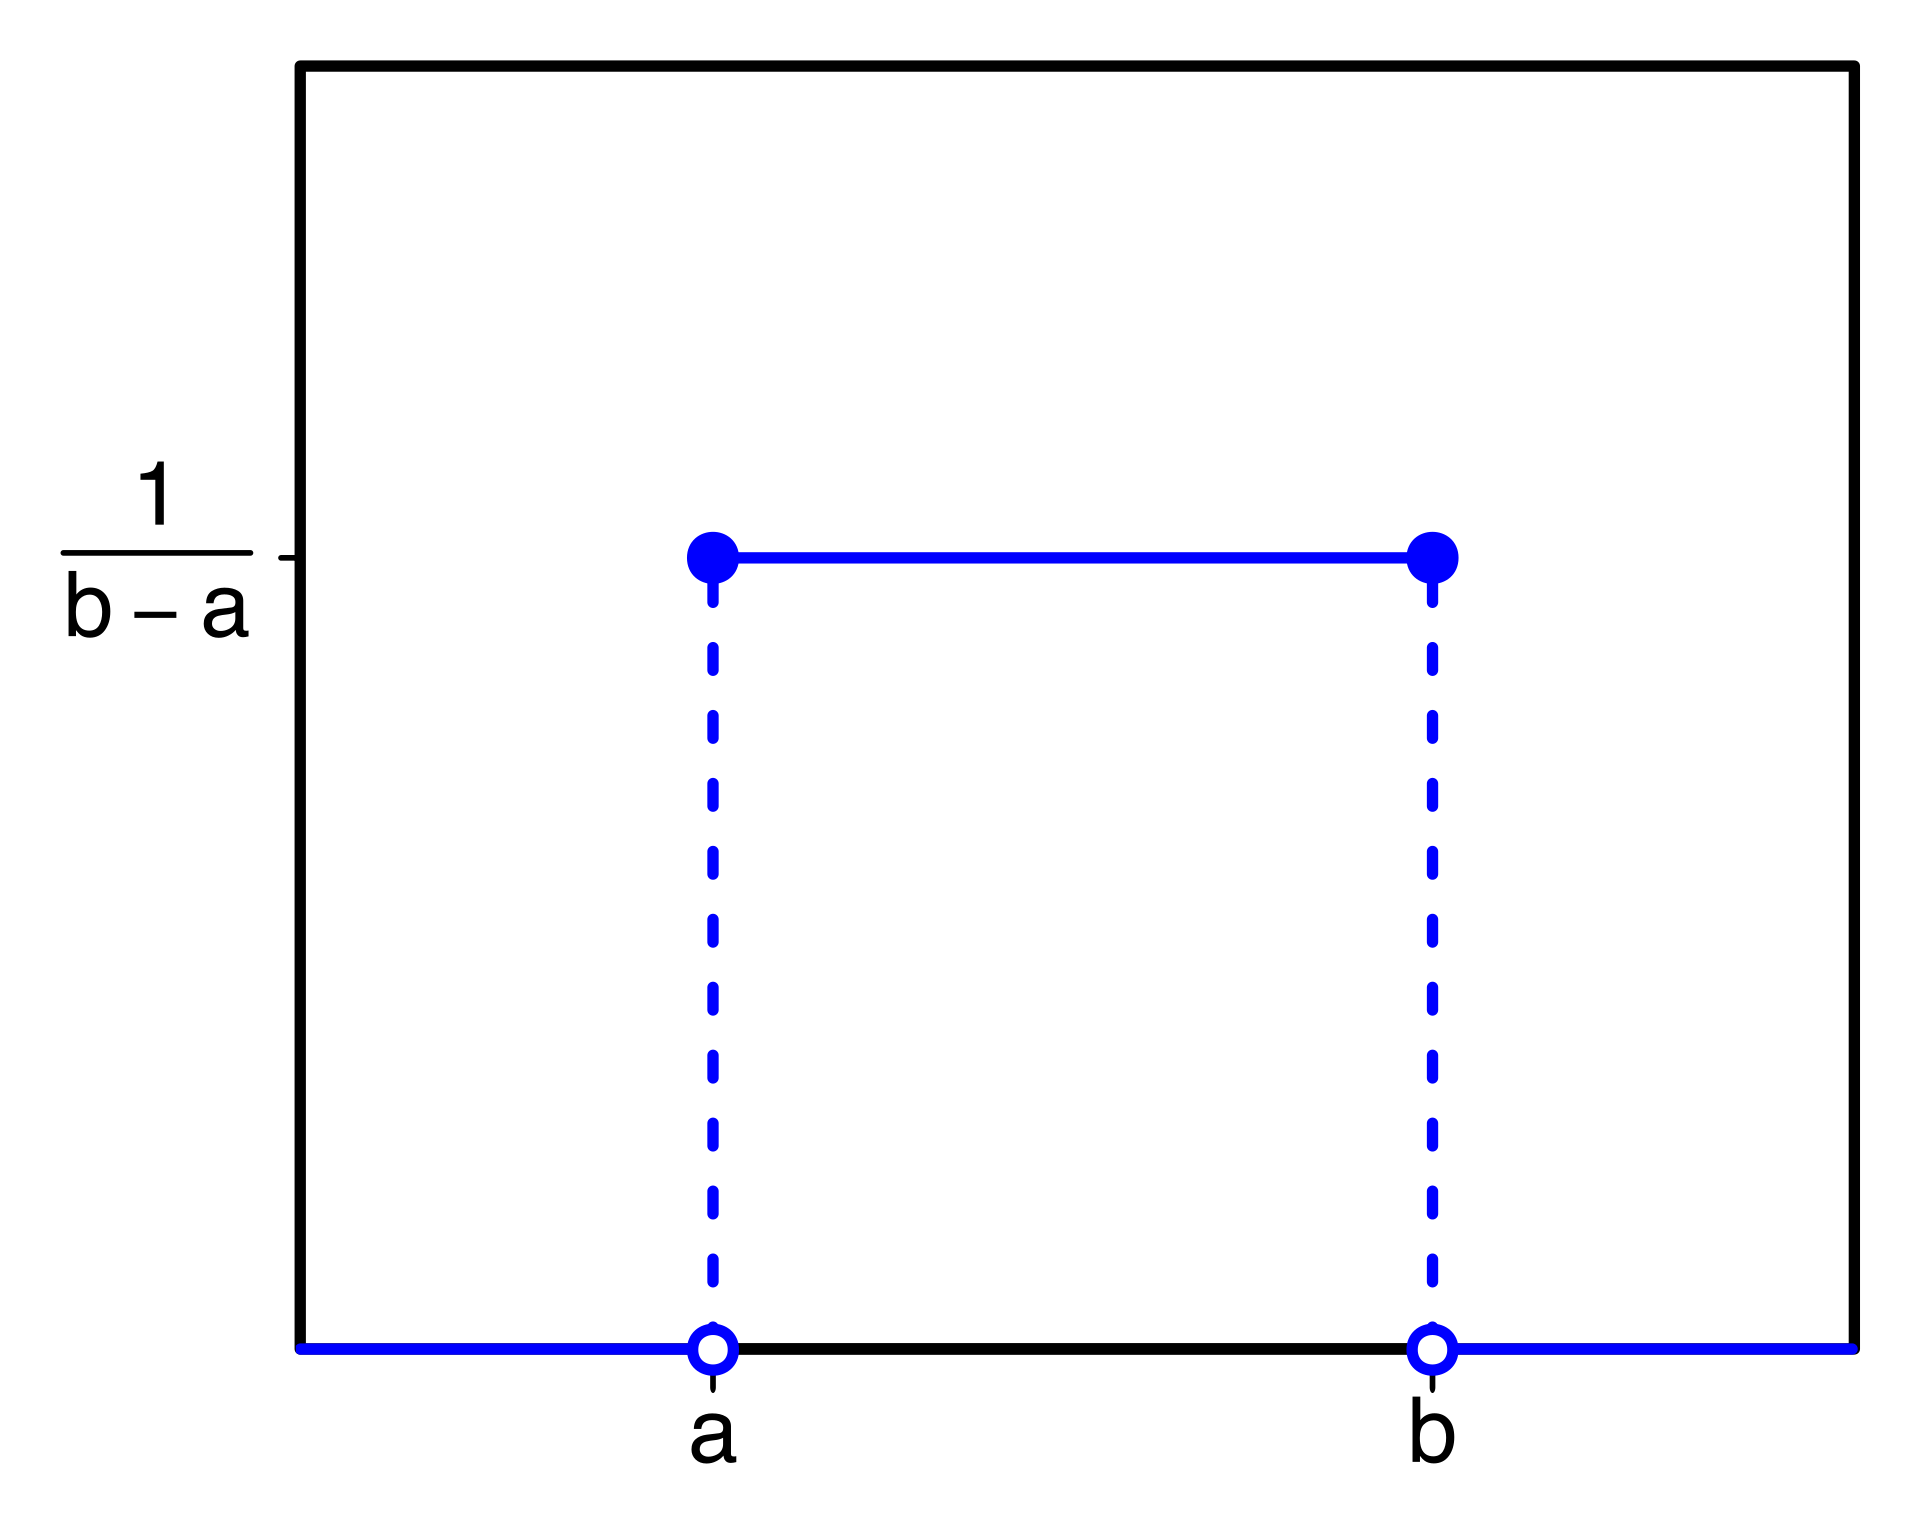
\includegraphics[width=0.5\linewidth]{assets/uni_f.png}
    \caption{Функция плотности равномерного распределения}
    \label{fig:}
    \end{center}
\end{figure}

\begin{figure}[H]
    \begin{center}
    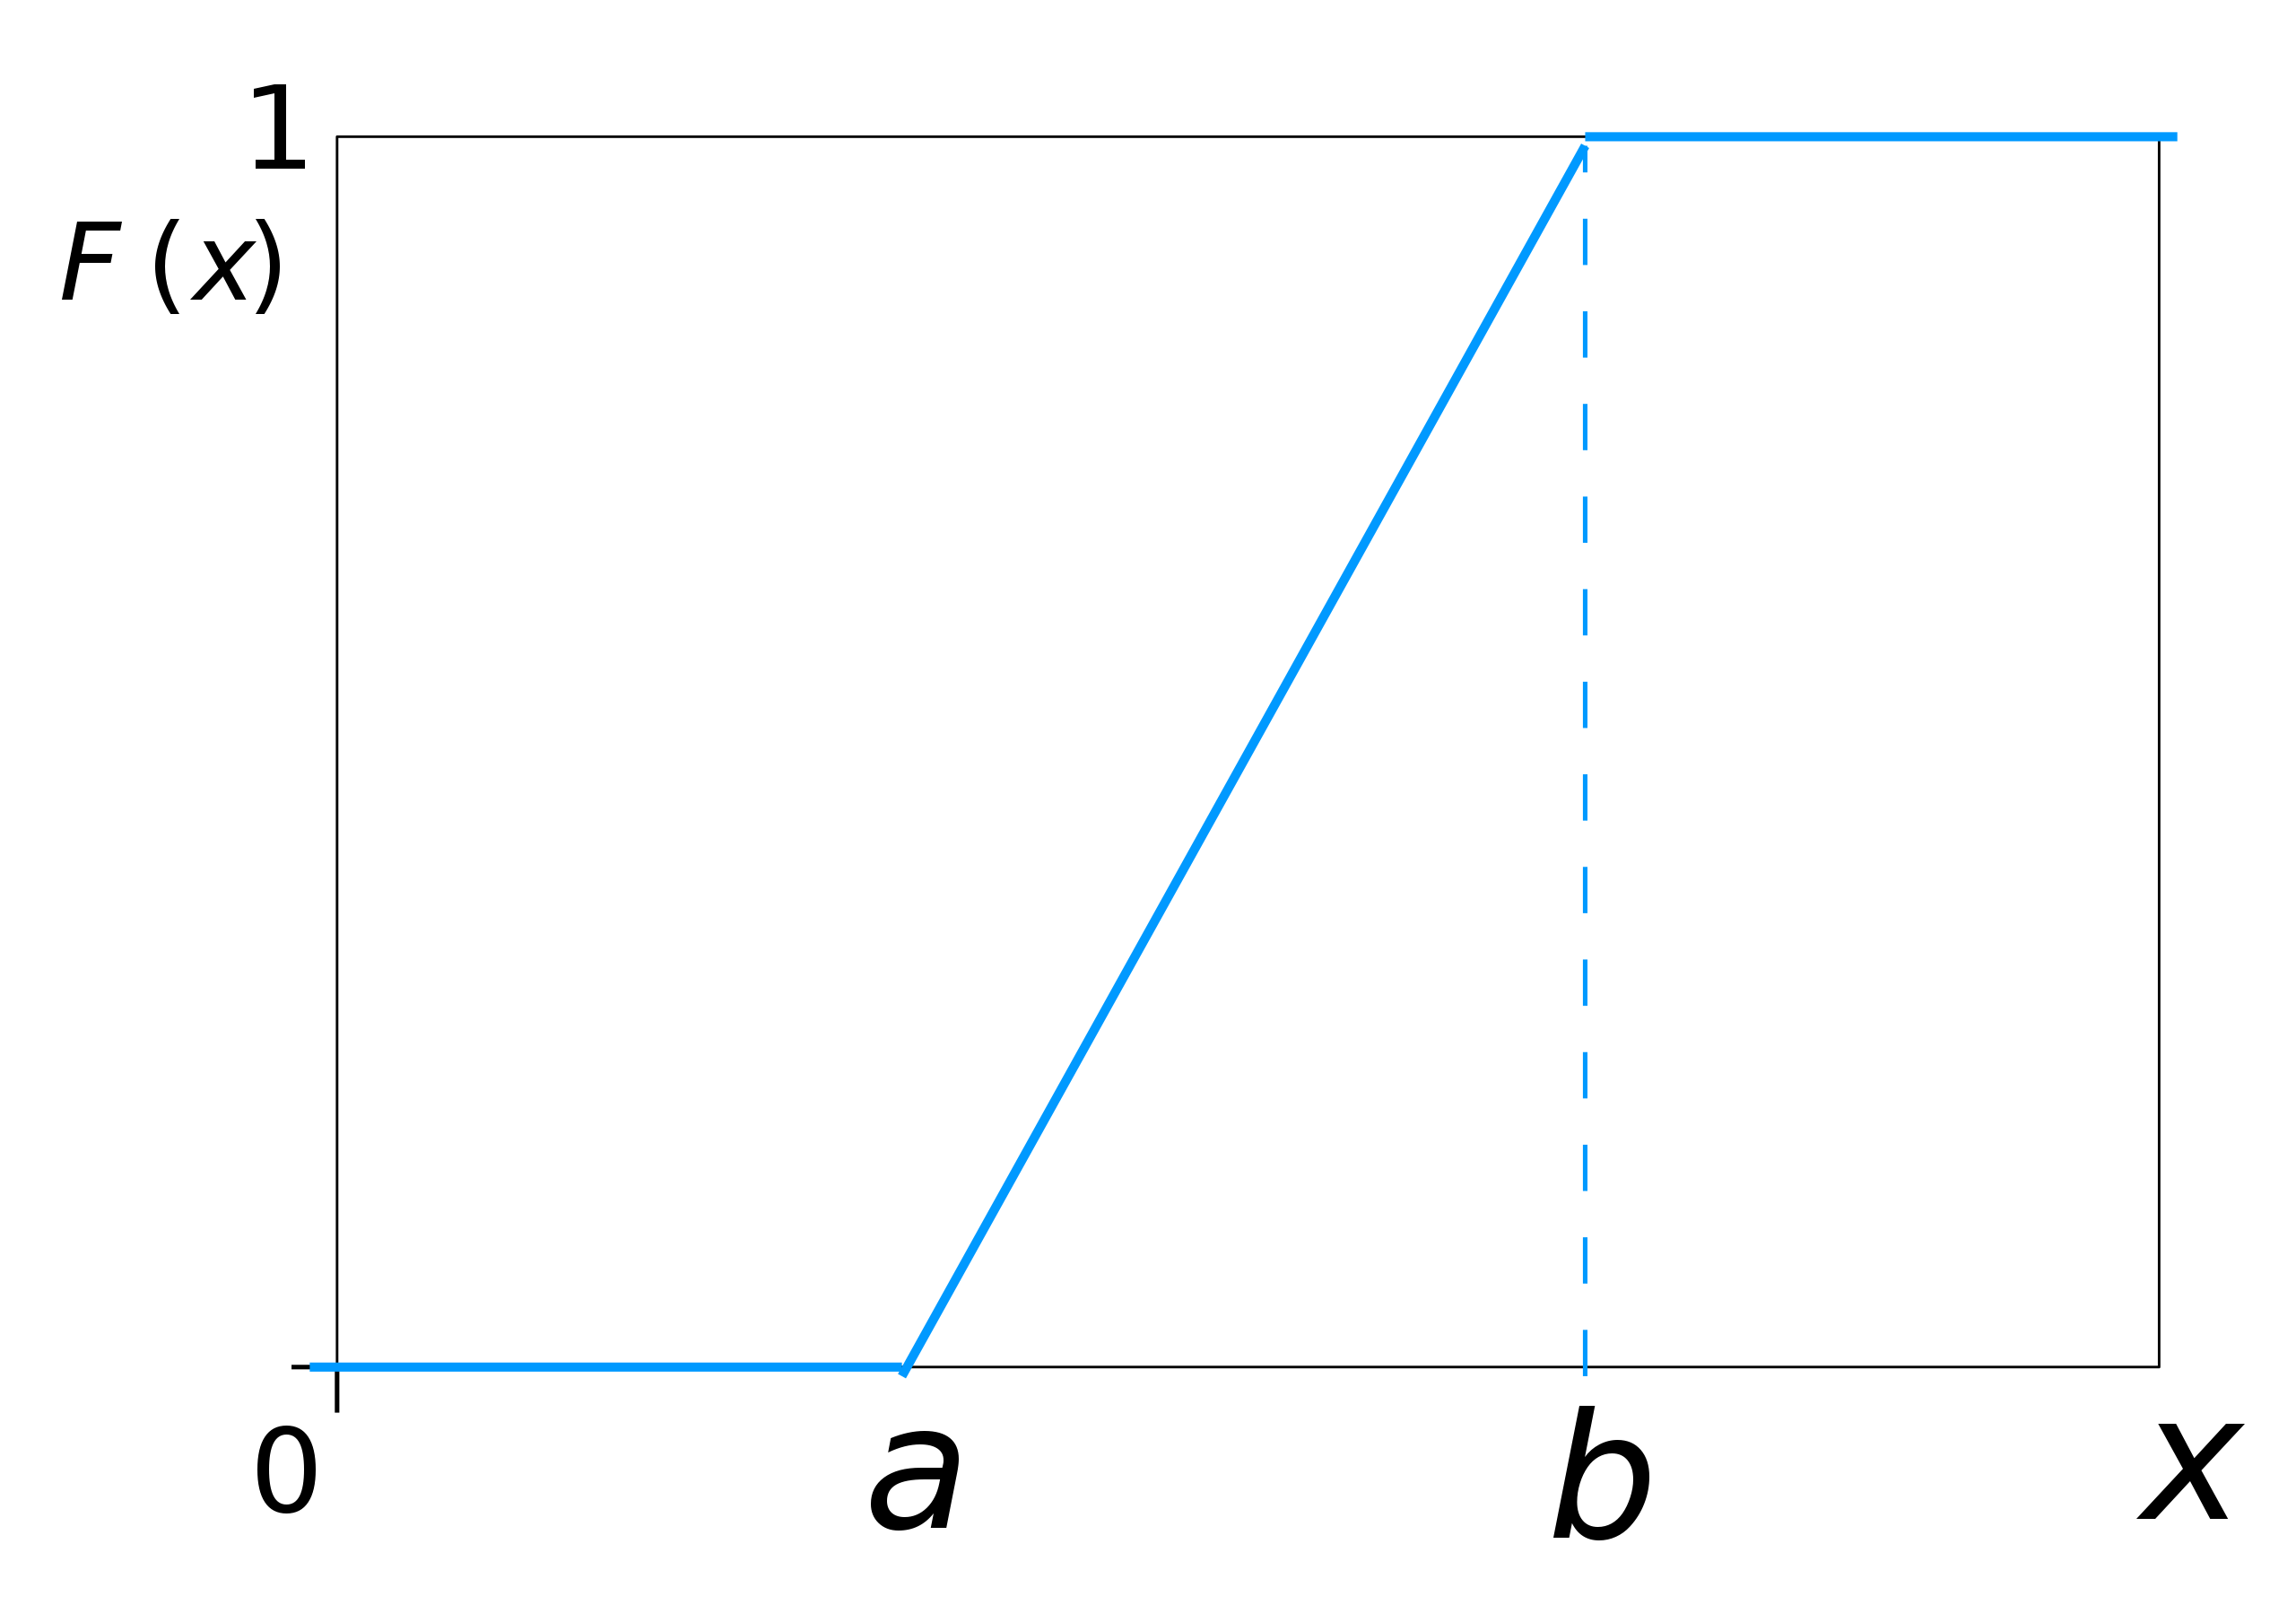
\includegraphics[width=0.5\linewidth]{assets/uni_Fx.png}
    \caption{Функция распределения равномерного распределения}
    \label{fig:}
    \end{center}
\end{figure}

\subsection{Распределение Эрланга}

Распределение Эрланга является непрерывным распределением, ограниченным снизу. Оно представляет собой особый случай Гамма распределения, где параметр $k$ может принимать только положительные целые значения.

Функция распределения:

\begin{equation*}
F_X(x) = 1 - \sum_{i=0}^{k-1}  \frac{1}{i!} e^{-\lambda x} (\lambda x)^n
\end{equation*}
    
Плотность распределения:

\begin{equation*}
f_X(x) = \frac{\lambda^k x^{k-1} e^{-\lambda x} } {(k-1)!}
\end{equation*}

\begin{figure}[H]
    \begin{center}
    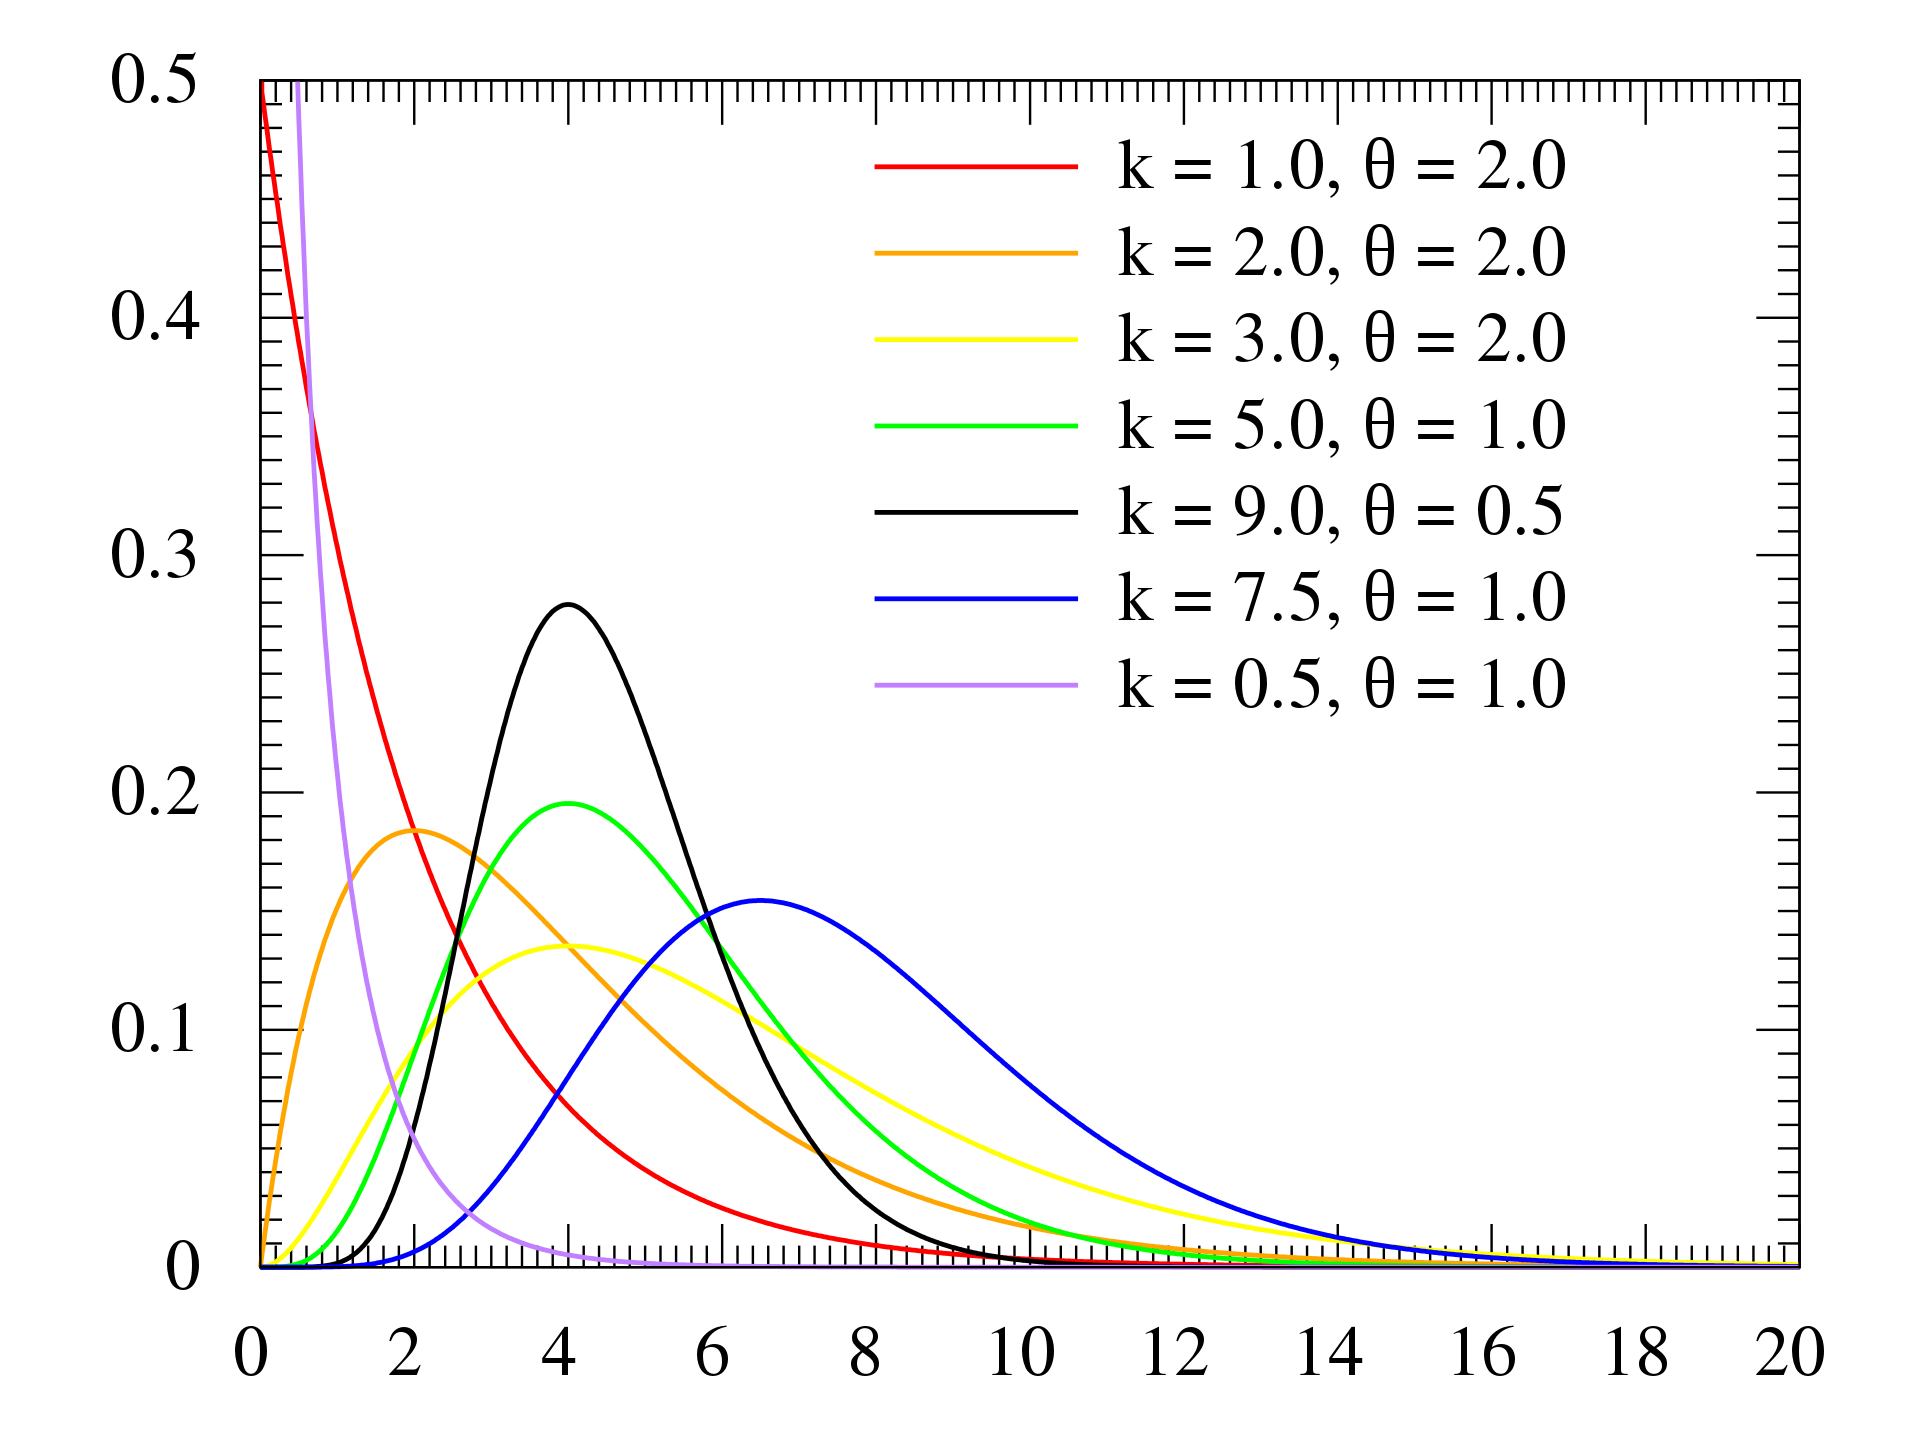
\includegraphics[width=0.5\linewidth]{assets/erlang_f.png}
    \caption{Функция плотности распределения Эрланга}
    \label{fig:}
    \end{center}
\end{figure}

\begin{figure}[H]
    \begin{center}
    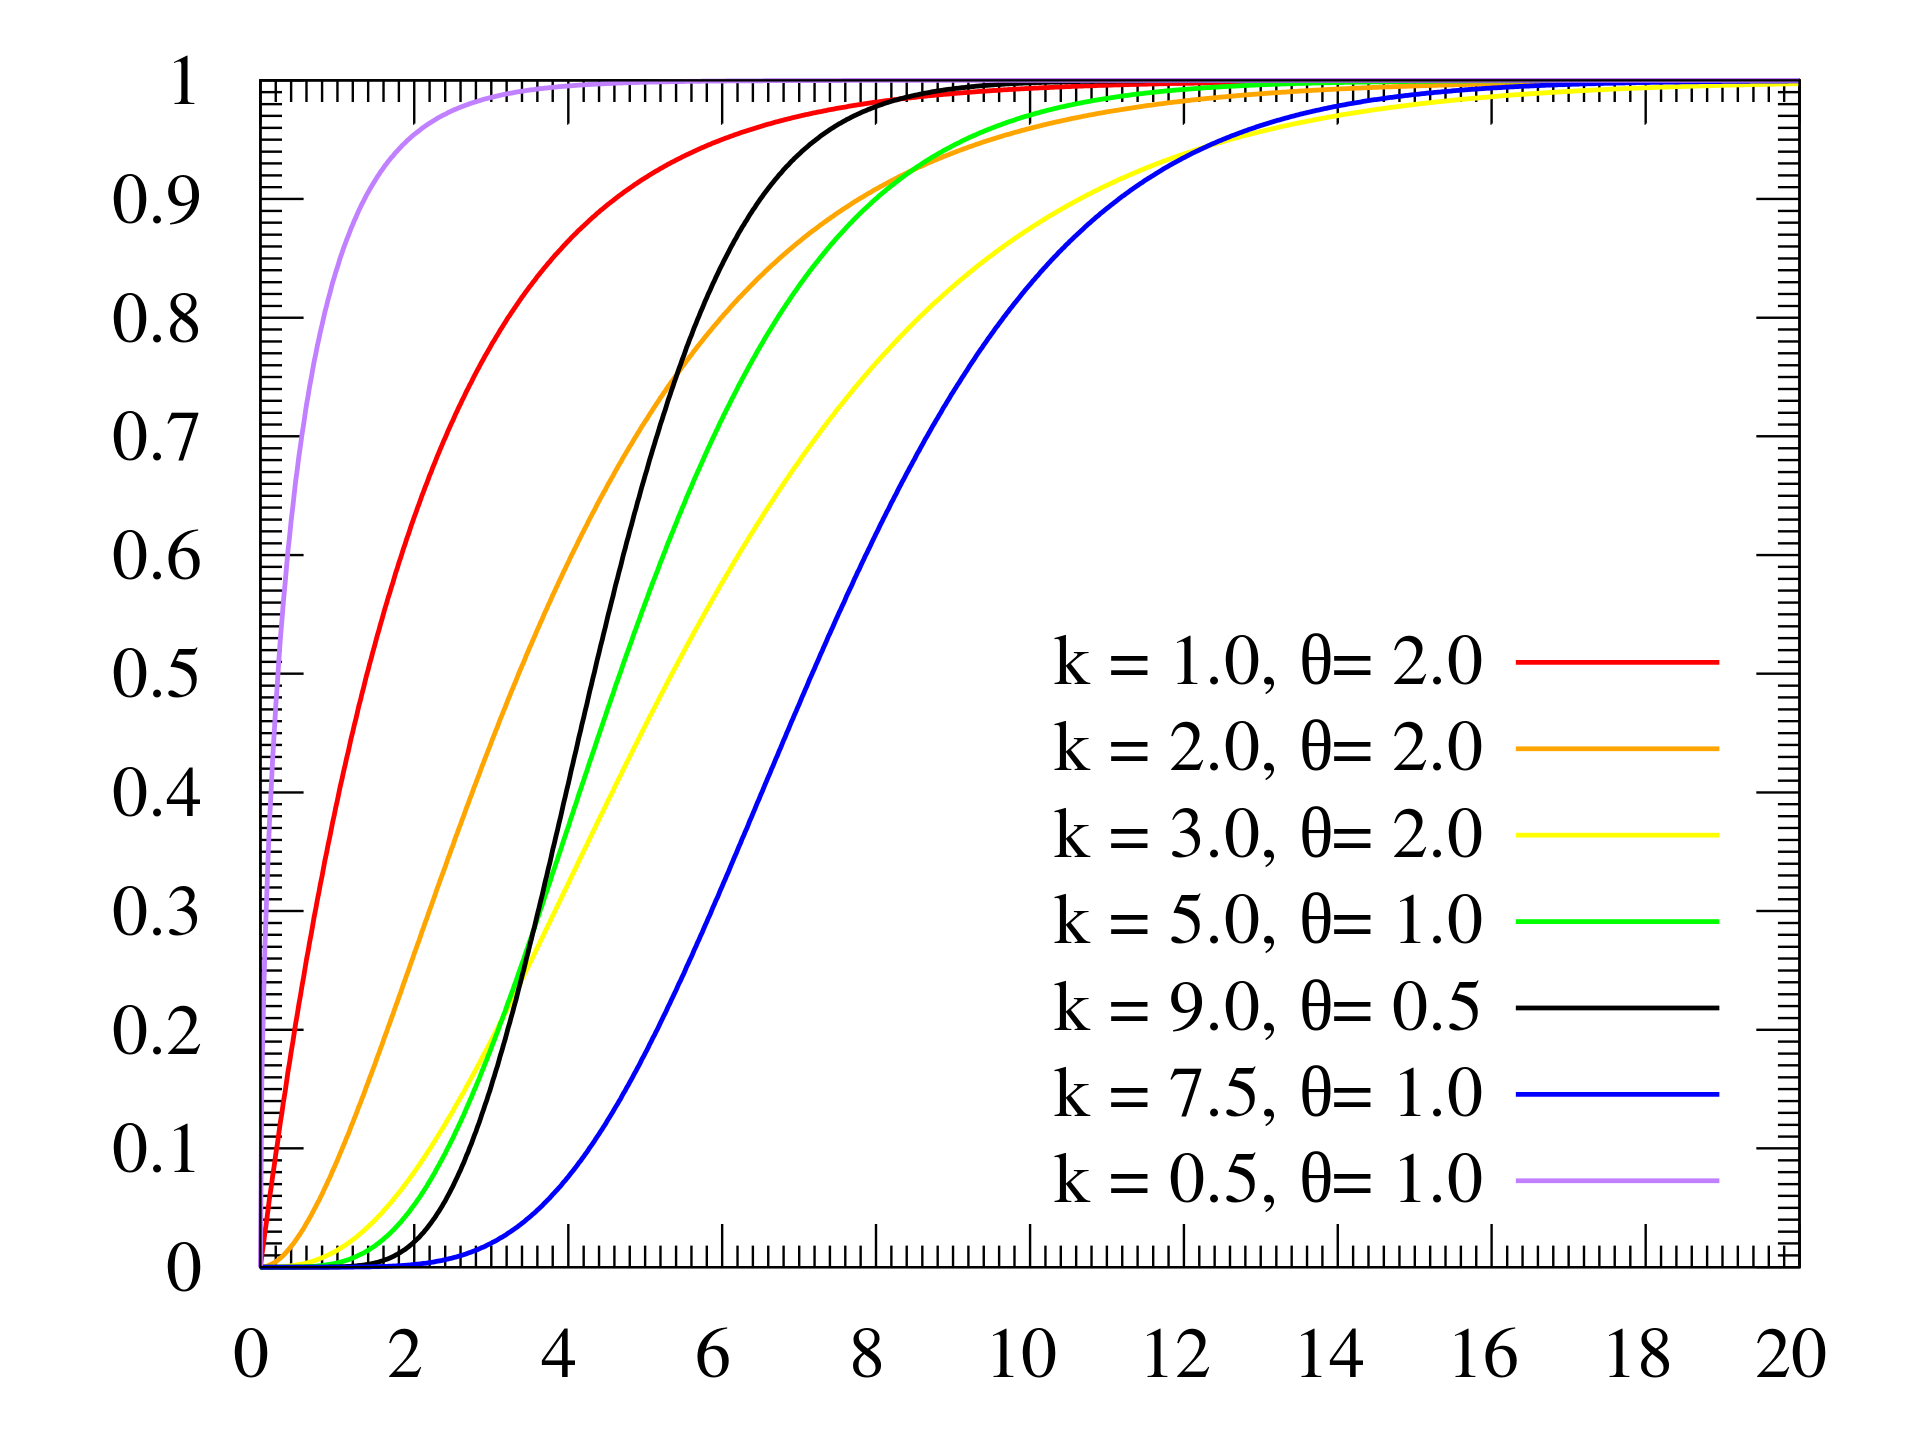
\includegraphics[width=0.5\linewidth]{assets/erlang_Fx.png}
    \caption{Функция распределения распределения Эрланга}
    \label{fig:}
    \end{center}
\end{figure}